\documentclass{article}

\usepackage{graphicx}
\usepackage{tikz}
\usepackage{tikzsymbols}
\usetikzlibrary{calc,patterns,shapes.geometric}
\pagestyle{empty}
\usepackage[margin=0pt]{geometry}
\geometry{papersize={14in,12in}}

\def\centerarc[#1](#2)(#3:#4:#5){\draw[#1] ($(#2)+({#5*cos(#3)},{#5*sin(#3)})$) arc (#3:#4:#5);}

\begin{document}
	\begin{figure}
		\centering
		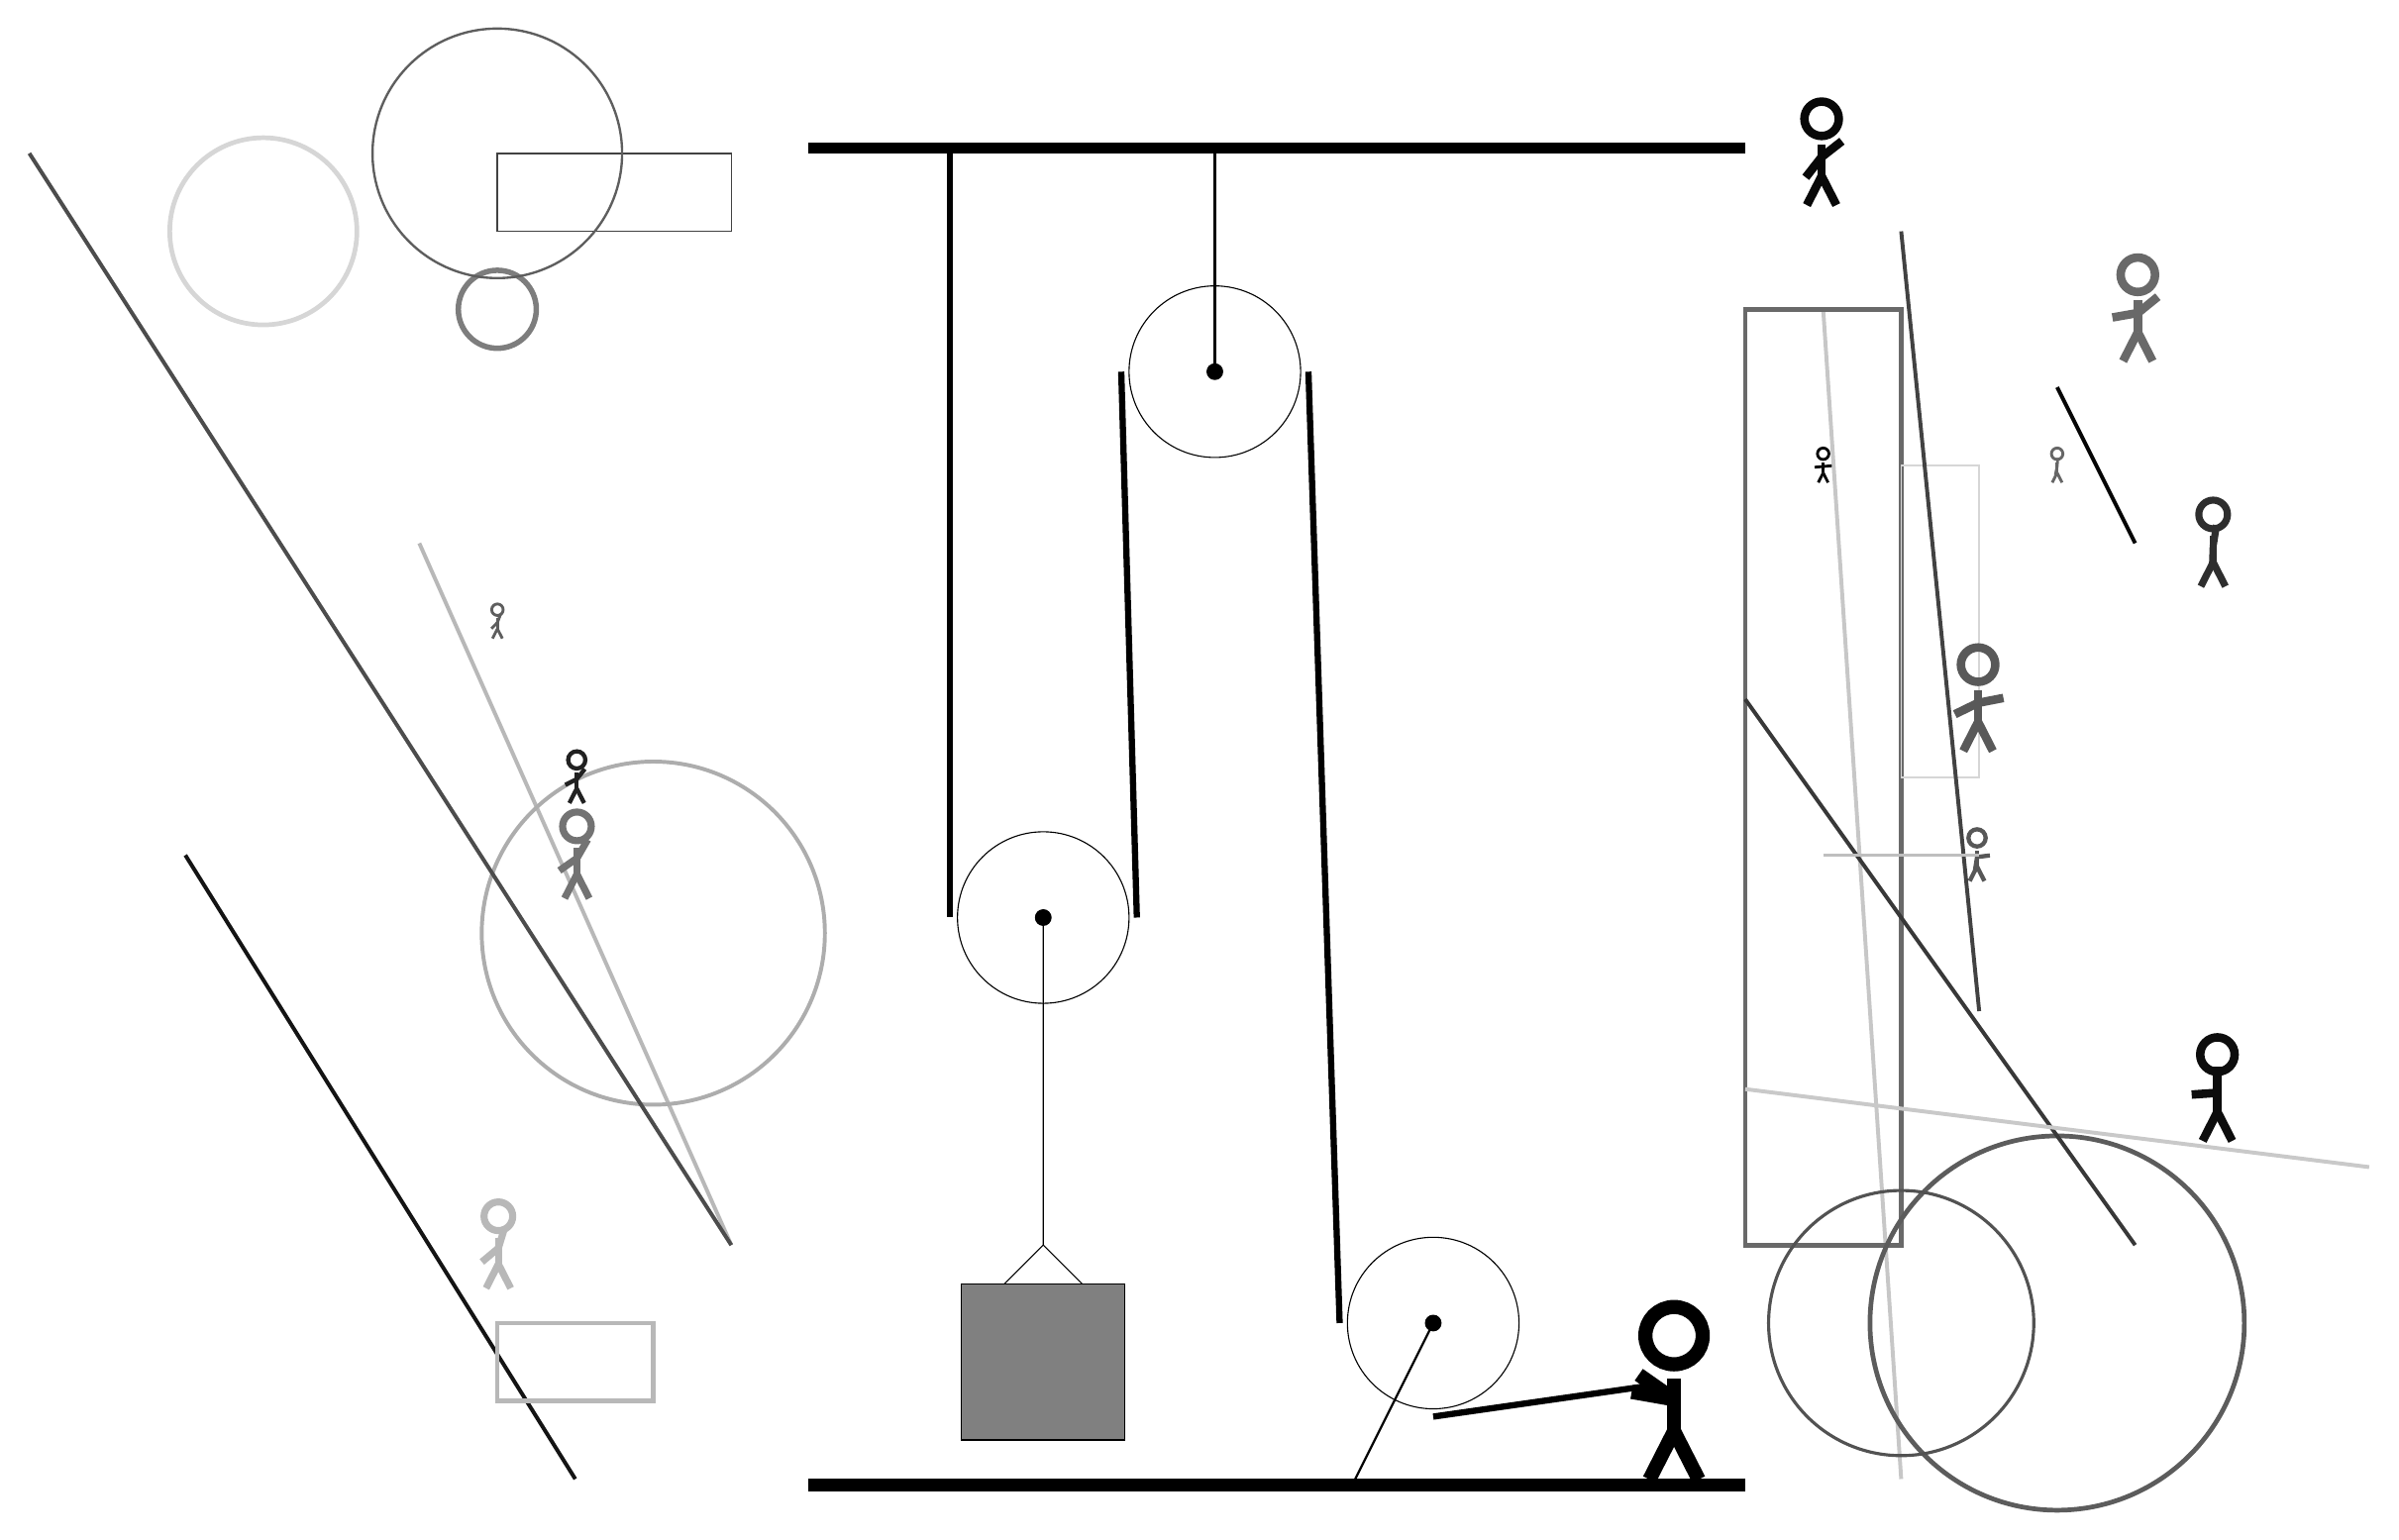
\begin{tikzpicture}
			%%%%% START %%%%%
			
			\draw[fill=black] (-2, 14) rectangle (10, 14.125);
			
			\draw (3.2, 11.2) circle (1.1);
			\draw[fill=black] (3.2, 11.2) circle (0.1);
			\draw[thick] (3.2, 11.2) -- (3.2, 14);
			
			\draw[line width=0.5mm, color=black!28](-7, 9) -- (-3, 0);
			
			\node[line width=0.7mm, color=black!59] at (15, 12) {\Strichmaxerl[6][10][39]};
			\draw [line width=0.6mm, color=black!16](-9, 13) circle (1.2);
			\draw [line width=0.7mm, color=black!51](-6, 12) circle (0.5);
			
			\node[line width=0.3mm, color=black!60] at (14, 10) {\Strichmaxerl[2][78][86]};
			\draw [line width=0.5mm, color=black!32](-4, 4) circle (2.2);
			\draw[line width=0.5mm, color=black!98](15, 9) -- (14, 11);
			\draw[line width=0.5mm, color=black!92](-5, -3) -- (-10, 5);
			\node[line width=0.4mm, color=black!66] at (13, 5) {\Strichmaxerl[3][81][7]};
			
			\draw[line width=0.5mm, color=black!22](11, 12) -- (12, -3);
			
			\node[line width=0.3mm, color=black!97] at (11, 14) {\Strichmaxerl[6][52][38]};
			
			\draw[line width=0.6mm, color=black!59] (12, 0) rectangle (10, 12);
			\node[line width=0.5mm, color=black!87] at (-5, 6) {\Strichmaxerl[3][27][51]};
			
			\node[line width=0.3mm, color=black!28] at (-6, 0) {\Strichmaxerl[5][40][73]};
			\draw [line width=0.6mm, color=black!64](14, -1) circle (2.4);
			\draw[line width=0.5mm, color=black!78](10, 7) -- (15, 0);
			
			\node[line width=0.3mm, color=black!97] at (11, 10) {\Strichmaxerl[2][5][5]};
			
			\draw[line width=0.2mm, color=black!16] (12, 10) rectangle (13, 6);
			\draw[line width=0.5mm, color=black!70](-3, 0) -- (-12, 14);
			
			\draw[line width=0.5mm, color=black!21](10, 2) -- (18, 1);
			\draw[line width=0.5mm, color=black!74](13, 3) -- (12, 13);
			
			\node[line width=0.3mm, color=black!82] at (16, 9) {\Strichmaxerl[5][88][81]};
			\draw[line width=0.6mm, color=black!28] (-4, -2) rectangle (-6, -1);
			\draw[line width=0.2mm, color=black!74] (-3, 13) rectangle (-6, 14);
			\draw [line width=0.3mm, color=black!63](-6, 14) circle (1.6);
			
			\node[line width=0.6mm, color=black!55] at (-5, 5) {\Strichmaxerl[5][35][60]};
			
			\draw [line width=0.4mm, color=black!68](12, -1) circle (1.7);
			\node[line width=0.7mm, color=black!65] at (13, 7) {\Strichmaxerl[6][26][11]};
			\node[line width=0.5mm, color=black!95] at (16, 2) {\Strichmaxerl[6][4][90]};
			\draw[line width=0.5mm, color=black!25](11, 5) -- (13, 5);
			\node[line width=0.7mm, color=black!63] at (-6, 8) {\Strichmaxerl[2][46][69]};
			
			
			\draw (6, -1) circle (1.1);
			\draw[fill=black] (6, -1) circle (0.1);
			\draw[thick] (6, -1) -- (5, -3);
			
			\draw (1, 4.2) circle (1.1);
			\draw[fill=black] (1, 4.2) circle (0.1);
			
			\draw (1, 4.2) -- (1, 0) -- (0.5, -0.5);
			\draw (1, 0) -- (1.5, -0.5);
			\draw[fill=black!50] (-0.05, -0.5) rectangle (2.05, -2.5);
			
			\draw[line width=0.8mm] (-0.2, 14) -- (-0.2, 4.2);
			\centerarc[line width=0.8mm](1, 4.2)(180:360:1.2000000000000002);
			\draw[line width=0.8mm](2.2, 4.2) -- (2.0, 11.2);
			\centerarc[line width=0.8mm](3.2, 11.2)(0:180:1.2000000000000002);
			\draw[line width=0.8mm](4.4, 11.2) -- (4.8, -1);
			\centerarc[line width=0.8mm](6, -1)(180:270:1.2000000000000002);
			\draw[line width=0.8mm](6, -2.2) -- (8.8, -1.8);
			
			\node at (9, -1.9) {\Strichmaxerl[10][-35][170]};
			
			\draw[fill=black] (-2, -3) rectangle (10, -3.15);
			
			%%%%% END %%%%%
		\end{tikzpicture}
	\end{figure}	
\end{document}